\section{Our Chip}
\label{sec:our_setup}

Our device consists of four star-shaped transmon qubits: two storage qubits and two emitters.
All of them are flux-tunable and thus coupled to a flux line.

\begin{figure}
    \centering
    \includegraphics[width = 1.\textwidth]{Images/Chap1/Uter_colorized_labels.png}
    \caption{False-color micrograph of the employed four-qubit device}
    \label{fig:our_chip}
\end{figure}

\subsection{Storage Qubits}
The storage qubits, depicted with an ‘S' in \cref{fig:our_chip}, are coupled to each other through a tunable coupler ($\text{C}_\text{S}$).
They have extended lifetimes, allowing us to execute multiple operations on them before they decay or suffer from decoherence.
The storage qubits are connected to both a readout resonator and a Purcell filter, for readout purposes.

\subsection{Readout resonator}

The readout mechanism comprises two primary components: the \emph{readout resonator} and the \emph{Purcell filter}. 
Its objective is to measure the state of the qubit in a non-destructive manner \cite{singleshot_readout}.

The starting point is the famous Jaynes-Cummings Hamiltonian \cite{haroche2006exploring}
\begin{equation}
    \hat{H} = \hbar \omega_r \hat{a}^\dagger \hat{a} + \frac{1}{2} \hbar \omega_{ge} \hat{\sigma}_z + \hbar g (\hat{a}^\dagger \hat{\sigma}^- + \hat{a} \hat{\sigma}^+) ,
\end{equation}
which models the interaction between a two-level system with transition frequency $\omega_{ge}$ and an electromagnetic field mode at frequency $\omega_r$.
In the dispersive regime ($|\omega_r - \omega_{ge} \gg g|$), the Hamiltonian reduces to \cite{transmon_regime}
\begin{align}
    \hat{H} &= \hbar \omega_r \hat{a}^\dagger \hat{a} + \frac{1}{2} \hbar \omega_{ge} \hat{\sigma}_z + \hbar \chi \hat{\sigma}_z \hat{a}^\dagger \hat{a} \\
    &= \hbar (\omega_r + \chi \hat{\sigma}_z ) \hat{a}^\dagger \hat{a} +
    \frac{1}{2} \hbar \omega_{ge} \hat{\sigma}_z 
\end{align}
where $\chi$ is the qubit-state dependent cavity-shift.

\begin{figure}
    \centering
    

\tikzset{every picture/.style={line width=0.75pt}} %set default line width to 0.75pt      

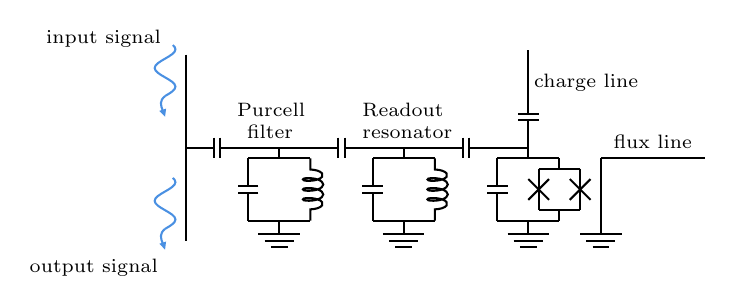
\begin{tikzpicture}[x=0.75pt,y=0.75pt,yscale=-1,xscale=1]
%uncomment if require: \path (0,300); %set diagram left start at 0, and has height of 300

%Shape: Capacitor [id:dp6229484510249941] 
\draw   (80,115) -- (93.5,115) (96.5,110) -- (96.5,120) (93.5,110) -- (93.5,120) (96.5,115) -- (110,115) ;
%Straight Lines [id:da5079772797363618] 
\draw    (140,120) -- (110,120) ;
%Shape: Inductor (Air Core) [id:dp10839806036975186] 
\draw   (140,120) -- (140,125.4) .. controls (142.63,125.48) and (144.87,126.23) .. (145.66,127.29) .. controls (146.44,128.35) and (145.61,129.5) .. (143.55,130.2) .. controls (141.95,130.74) and (139.88,130.95) .. (137.87,130.8) .. controls (137.08,130.8) and (136.45,130.53) .. (136.45,130.2) .. controls (136.45,129.87) and (137.08,129.6) .. (137.87,129.6) .. controls (139.88,129.45) and (141.95,129.66) .. (143.55,130.2) .. controls (145.26,130.82) and (146.23,131.69) .. (146.23,132.6) .. controls (146.23,133.51) and (145.26,134.38) .. (143.55,135) .. controls (141.95,135.54) and (139.88,135.75) .. (137.87,135.6) .. controls (137.08,135.6) and (136.45,135.33) .. (136.45,135) .. controls (136.45,134.67) and (137.08,134.4) .. (137.87,134.4) .. controls (139.88,134.25) and (141.95,134.46) .. (143.55,135) .. controls (145.26,135.62) and (146.23,136.49) .. (146.23,137.4) .. controls (146.23,138.31) and (145.26,139.18) .. (143.55,139.8) .. controls (141.95,140.34) and (139.88,140.55) .. (137.87,140.4) .. controls (137.08,140.4) and (136.45,140.13) .. (136.45,139.8) .. controls (136.45,139.47) and (137.08,139.2) .. (137.87,139.2) .. controls (139.88,139.05) and (141.95,139.26) .. (143.55,139.8) .. controls (145.61,140.5) and (146.44,141.65) .. (145.66,142.71) .. controls (144.87,143.77) and (142.63,144.52) .. (140,144.6) -- (140,150) ;
%Shape: Capacitor [id:dp06818692783071034] 
\draw   (110,120) -- (110,133.5) (115,136.5) -- (105,136.5) (115,133.5) -- (105,133.5) (110,136.5) -- (110,150) ;
%Straight Lines [id:da7350026547264685] 
\draw    (110,150) -- (140,150) ;
%Straight Lines [id:da23995913734624486] 
\draw    (80,70) -- (80,160) ;
%Straight Lines [id:da1612492392898659] 
\draw    (110,115) -- (140,115) ;
%Straight Lines [id:da5671640840709973] 
\draw    (125,115) -- (125,120) ;
%Shape: Capacitor [id:dp5438650003798182] 
\draw   (140,115) -- (153.5,115) (156.5,110) -- (156.5,120) (153.5,110) -- (153.5,120) (156.5,115) -- (170,115) ;
%Straight Lines [id:da49049414599623864] 
\draw    (200,120) -- (170,120) ;
%Shape: Inductor (Air Core) [id:dp010409349579149074] 
\draw   (200,120) -- (200,125.4) .. controls (202.63,125.48) and (204.87,126.23) .. (205.66,127.29) .. controls (206.44,128.35) and (205.61,129.5) .. (203.55,130.2) .. controls (201.95,130.74) and (199.88,130.95) .. (197.87,130.8) .. controls (197.08,130.8) and (196.45,130.53) .. (196.45,130.2) .. controls (196.45,129.87) and (197.08,129.6) .. (197.87,129.6) .. controls (199.88,129.45) and (201.95,129.66) .. (203.55,130.2) .. controls (205.26,130.82) and (206.23,131.69) .. (206.23,132.6) .. controls (206.23,133.51) and (205.26,134.38) .. (203.55,135) .. controls (201.95,135.54) and (199.88,135.75) .. (197.87,135.6) .. controls (197.08,135.6) and (196.45,135.33) .. (196.45,135) .. controls (196.45,134.67) and (197.08,134.4) .. (197.87,134.4) .. controls (199.88,134.25) and (201.95,134.46) .. (203.55,135) .. controls (205.26,135.62) and (206.23,136.49) .. (206.23,137.4) .. controls (206.23,138.31) and (205.26,139.18) .. (203.55,139.8) .. controls (201.95,140.34) and (199.88,140.55) .. (197.87,140.4) .. controls (197.08,140.4) and (196.45,140.13) .. (196.45,139.8) .. controls (196.45,139.47) and (197.08,139.2) .. (197.87,139.2) .. controls (199.88,139.05) and (201.95,139.26) .. (203.55,139.8) .. controls (205.61,140.5) and (206.44,141.65) .. (205.66,142.71) .. controls (204.87,143.77) and (202.63,144.52) .. (200,144.6) -- (200,150) ;
%Shape: Capacitor [id:dp38289405277156474] 
\draw   (170,120) -- (170,133.5) (175,136.5) -- (165,136.5) (175,133.5) -- (165,133.5) (170,136.5) -- (170,150) ;
%Straight Lines [id:da7342631646168638] 
\draw    (170,150) -- (200,150) ;
%Shape: Capacitor [id:dp4965705456609162] 
\draw   (200,115) -- (213.5,115) (216.5,110) -- (216.5,120) (213.5,110) -- (213.5,120) (216.5,115) -- (230,115) ;
%Straight Lines [id:da5477595668599946] 
\draw    (170,115) -- (200,115) ;
%Straight Lines [id:da7609436744451872] 
\draw    (185,115) -- (185,120) ;
%Straight Lines [id:da932132356010352] 
\draw    (260,120) -- (230,120) ;
%Shape: Capacitor [id:dp925083204210299] 
\draw   (230,120) -- (230,133.5) (235,136.5) -- (225,136.5) (235,133.5) -- (225,133.5) (230,136.5) -- (230,150) ;
%Straight Lines [id:da48756322841661204] 
\draw    (230,150) -- (260,150) ;
%Straight Lines [id:da9662762169593431] 
\draw    (245,115) -- (245,120) ;
%Straight Lines [id:da607486087129423] 
\draw    (250,125) -- (270,125) ;
%Straight Lines [id:da4269839144692542] 
\draw    (250,145) -- (270,145) ;
%Straight Lines [id:da6212379775483154] 
\draw    (270,125) -- (270,145) ;
%Straight Lines [id:da42941601462568646] 
\draw    (250,125) -- (250,145) ;
%Straight Lines [id:da9671029825944342] 
\draw    (260,120) -- (260,125) ;
%Straight Lines [id:da9712181495027408] 
\draw    (260,145) -- (260,150) ;
%Straight Lines [id:da3624697790998732] 
\draw    (265,130) -- (275,140) ;
%Straight Lines [id:da4335724022567018] 
\draw    (245,130) -- (255,140) ;
%Straight Lines [id:da530417781084312] 
\draw    (255,130) -- (245,140) ;
%Straight Lines [id:da9581131846208597] 
\draw    (275,130) -- (265,140) ;
%Straight Lines [id:da038301723534536425] 
\draw    (230,115) -- (245,115) ;
%Shape: Ground [id:dp6910953506421662] 
\draw   (115,156.67) -- (135,156.67) ;
\draw   (118,159.67) -- (132,159.67) ;
\draw   (121,162.67) -- (129,162.67) ;
\draw   (125,150) -- (125,156.67) ;
%Shape: Ground [id:dp4840755871676472] 
\draw   (175,156.67) -- (195,156.67) ;
\draw   (178,159.67) -- (192,159.67) ;
\draw   (181,162.67) -- (189,162.67) ;
\draw   (185,150) -- (185,156.67) ;
%Shape: Ground [id:dp7159028270026297] 
\draw   (235,156.67) -- (255,156.67) ;
\draw   (238,159.67) -- (252,159.67) ;
\draw   (241,162.67) -- (249,162.67) ;
\draw   (245,150) -- (245,156.67) ;
%Straight Lines [id:da07274023253816075] 
\draw    (280,120) -- (330,120) ;
%Straight Lines [id:da0646328748380458] 
\draw    (280,120) -- (280,150) ;
%Shape: Ground [id:dp10990759893272828] 
\draw   (270,156.67) -- (290,156.67) ;
\draw   (273,159.67) -- (287,159.67) ;
\draw   (276,162.67) -- (284,162.67) ;
\draw   (280,150) -- (280,156.67) ;
%Straight Lines [id:da8443452176258857] 
\draw    (245,68) -- (245,85) ;
%Shape: Capacitor [id:dp2673784375807502] 
\draw   (245,85) -- (245,98.5) (250,101.5) -- (240,101.5) (250,98.5) -- (240,98.5) (245,101.5) -- (245,115) ;
%Shape: Wave [id:dp46962992426174544] 
\draw  [color={rgb, 255:red, 74; green, 144; blue, 226 }  ,draw opacity=1 ] (70,90) .. controls (72.56,88.53) and (75,87.13) .. (75,85.5) .. controls (75,83.87) and (72.56,82.47) .. (70,81) .. controls (67.44,79.53) and (65,78.13) .. (65,76.5) .. controls (65,74.87) and (67.44,73.47) .. (70,72) .. controls (72.56,70.53) and (75,69.13) .. (75,67.5) .. controls (75,66.77) and (74.51,66.09) .. (73.75,65.43) ;
%Curve Lines [id:da8193635142444085] 
\draw [color={rgb, 255:red, 74; green, 144; blue, 226 }  ,draw opacity=1 ]   (70,90) .. controls (67.21,92.34) and (67.82,94.25) .. (68.96,97.21) ;
\draw [shift={(70,100)}, rotate = 251.57] [fill={rgb, 255:red, 74; green, 144; blue, 226 }  ,fill opacity=1 ][line width=0.08]  [draw opacity=0] (3.57,-1.72) -- (0,0) -- (3.57,1.72) -- cycle    ;
%Shape: Wave [id:dp5292058745377288] 
\draw  [color={rgb, 255:red, 74; green, 144; blue, 226 }  ,draw opacity=1 ] (70,154) .. controls (72.56,152.53) and (75,151.13) .. (75,149.5) .. controls (75,147.87) and (72.56,146.47) .. (70,145) .. controls (67.44,143.53) and (65,142.13) .. (65,140.5) .. controls (65,138.87) and (67.44,137.47) .. (70,136) .. controls (72.56,134.53) and (75,133.13) .. (75,131.5) .. controls (75,130.77) and (74.51,130.09) .. (73.75,129.43) ;
%Curve Lines [id:da04097203302843688] 
\draw [color={rgb, 255:red, 74; green, 144; blue, 226 }  ,draw opacity=1 ]   (70,154) .. controls (67.21,156.34) and (67.82,158.25) .. (68.96,161.21) ;
\draw [shift={(70,164)}, rotate = 251.57] [fill={rgb, 255:red, 74; green, 144; blue, 226 }  ,fill opacity=1 ][line width=0.08]  [draw opacity=0] (3.57,-1.72) -- (0,0) -- (3.57,1.72) -- cycle    ;

% Text Node
\draw (305,117) node [anchor=south] [inner sep=0.75pt]  [font=\scriptsize] [align=left] {{\scriptsize flux line}};
% Text Node
\draw (246.31,83.64) node [anchor=west] [inner sep=0.75pt]  [font=\scriptsize] [align=left] {{\scriptsize charge line}};
% Text Node
\draw (181,112) node [anchor=south] [inner sep=0.75pt]  [font=\scriptsize] [align=left] {\begin{minipage}[lt]{23.84pt}\setlength\topsep{0pt}
\begin{center}
{\scriptsize Readout}\\{\scriptsize resonator }
\end{center}

\end{minipage}};
% Text Node
\draw (138,112) node [anchor=south east] [inner sep=0.75pt]  [font=\scriptsize] [align=left] {\begin{minipage}[lt]{23.84pt}\setlength\topsep{0pt}
\begin{center}
{\scriptsize Purcell}\\{\scriptsize filter}
\end{center}

\end{minipage}};
% Text Node
\draw (69.47,67.86) node [anchor=south east] [inner sep=0.75pt]  [font=\scriptsize] [align=left] {{\scriptsize input signal}};
% Text Node
\draw (68,167) node [anchor=north east] [inner sep=0.75pt]  [font=\scriptsize] [align=left] {{\scriptsize output signal}};


\end{tikzpicture}


    \vspace{-1cm}
    \caption{Diagram representing a qubit together with flux line, charge line and readout mechanism}
    \label{fig:diagram_storage_qubit}
\end{figure}

Thus, the resonator's frequency becomes qubit-state's dependent.
If, for instance, the qubit is in the $\ket{g}$ state, then the resonator's frequency will become $\omega_r - \chi$.
On the other hand, if the qubit is in the $\ket{e}$ state, then the resonator's frequency will be $\omega_r + \chi$.
The frequency of the resonator can be determined by assessing the transmission of an input signal through the feedline (see \cref{fig:diagram_storage_qubit}).
This transmission decreases when the signal is on resonance with the resonator's frequency.

In case where the qubit is in a mixed state like
\begin{equation}
    c_g \ket{g} + c_e \ket{e} ,
\end{equation}
then driving the resonator would results in an entangled state between the coherent signal and the qubit
\begin{equation}
    c_g \ket{g, \alpha_g} + c_e \ket{e, \alpha_e} .
\end{equation}
Thus, measuring either $\alpha_g$ or $\alpha_e$ will collapse the state of the qubit onto $\ket{g}$ or $\ket{e}$, respectively.
The principle underlying quantum non-demolition (QND) measurement is predicated on the stability of the state post-measurement.
This implies that subsequent QND measurements would yield identical results, as the state remains unchanged.

To prevent excessive coupling between the qubit and its environment via the readout resonator, a Purcell filter is interposed between them.
This configuration helps extend the qubit lifetimes by mitigating spontaneous emission resulting from the Purcell effect \cite{Purcell_effect}.

\subsection{Tunable couplers}

\begin{figure}[b]
    \centering
    \begin{subfigure}{0.65\textwidth}
        \centering
        

\tikzset{every picture/.style={line width=0.75pt}} %set default line width to 0.75pt        

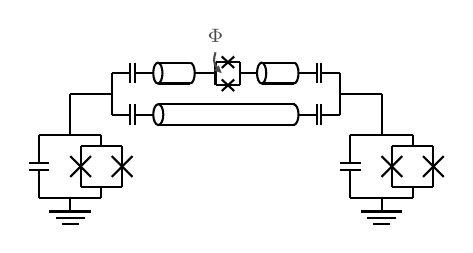
\begin{tikzpicture}[x=0.75pt,y=0.75pt,yscale=-1,xscale=1]
%uncomment if require: \path (0,300); %set diagram left start at 0, and has height of 300

%Straight Lines [id:da07218492708859259] 
\draw    (165,140) -- (135,140) ;
%Shape: Capacitor [id:dp26518043172092054] 
\draw   (135,140) -- (135,153.5) (140,156.5) -- (130,156.5) (140,153.5) -- (130,153.5) (135,156.5) -- (135,170) ;
%Straight Lines [id:da13302415031214743] 
\draw    (135,170) -- (165,170) ;
%Straight Lines [id:da17130629114618245] 
\draw    (155,145) -- (175,145) ;
%Straight Lines [id:da29260280538604033] 
\draw    (155,165) -- (175,165) ;
%Straight Lines [id:da49230231307780326] 
\draw    (175,145) -- (175,165) ;
%Straight Lines [id:da3653947605727903] 
\draw    (155,145) -- (155,165) ;
%Straight Lines [id:da44803766219329755] 
\draw    (165,140) -- (165,145) ;
%Straight Lines [id:da9101556277746032] 
\draw    (165,165) -- (165,170) ;
%Straight Lines [id:da006475878830819681] 
\draw    (170,150) -- (180,160) ;
%Straight Lines [id:da33120831736226397] 
\draw    (150,150) -- (160,160) ;
%Straight Lines [id:da11004761294731558] 
\draw    (160,150) -- (150,160) ;
%Straight Lines [id:da9445264009597942] 
\draw    (180,150) -- (170,160) ;
%Shape: Ground [id:dp22167919288849824] 
\draw   (140, 176.67) -- (160, 176.67) ;
\draw   (143, 179.67) -- (157, 179.67) ;
\draw   (146, 182.67) -- (154, 182.67) ;
\draw   (150, 170) -- (150, 176.67) ;
%Straight Lines [id:da42940827257352] 
\draw    (315,140) -- (285,140) ;
%Shape: Capacitor [id:dp49877304955829627] 
\draw   (285,140) -- (285,153.5) (290,156.5) -- (280,156.5) (290,153.5) -- (280,153.5) (285,156.5) -- (285,170) ;
%Straight Lines [id:da7324100328789034] 
\draw    (285,170) -- (315,170) ;
%Straight Lines [id:da208048098521316] 
\draw    (305,145) -- (325,145) ;
%Straight Lines [id:da8572518030578566] 
\draw    (305,165) -- (325,165) ;
%Straight Lines [id:da5742858039200953] 
\draw    (325,145) -- (325,165) ;
%Straight Lines [id:da3966431831849069] 
\draw    (305,145) -- (305,165) ;
%Straight Lines [id:da19183525795672862] 
\draw    (315,140) -- (315,145) ;
%Straight Lines [id:da004743615923411104] 
\draw    (315,165) -- (315,170) ;
%Straight Lines [id:da17738152912719607] 
\draw    (320,150) -- (330,160) ;
%Straight Lines [id:da8678835567326026] 
\draw    (300,150) -- (310,160) ;
%Straight Lines [id:da28374358820735224] 
\draw    (310,150) -- (300,160) ;
%Straight Lines [id:da24817307713778236] 
\draw    (330,150) -- (320,160) ;
%Shape: Ground [id:dp861700376356459] 
\draw   (290, 176.67) -- (310, 176.67) ;
\draw   (293, 179.67) -- (307, 179.67) ;
\draw   (296, 182.67) -- (304, 182.67) ;
\draw   (300, 170) -- (300, 176.67) ;
%Straight Lines [id:da6625685419222695] 
\draw    (150,140) -- (150,120) ;
%Straight Lines [id:da2635718281625268] 
\draw    (300,140) -- (300,120) ;
%Straight Lines [id:da3980890926472094] 
\draw    (170,120) -- (150,120) ;
%Straight Lines [id:da6516978234304753] 
\draw    (170,120) -- (170,110) ;
%Straight Lines [id:da8682527218489697] 
\draw    (170,130) -- (170,120) ;
%Shape: Capacitor [id:dp26464751353501326] 
\draw   (170,110) -- (179,110) (181,105) -- (181,115) (179,105) -- (179,115) (181,110) -- (190,110) ;
%Shape: Capacitor [id:dp9673816527519772] 
\draw   (170,130) -- (179,130) (181,125) -- (181,135) (179,125) -- (179,135) (181,130) -- (190,130) ;
%Shape: Ellipse [id:dp26511497109868176] 
\draw   (190,110) .. controls (190,107.24) and (191,105) .. (192.22,105) .. controls (193.45,105) and (194.45,107.24) .. (194.45,110) .. controls (194.45,112.76) and (193.45,115) .. (192.22,115) .. controls (191,115) and (190,112.76) .. (190,110) -- cycle ;
%Straight Lines [id:da14470289747688758] 
\draw    (192.22,105) -- (207.79,105) ;
%Straight Lines [id:da773223714503521] 
\draw    (192.22,115) -- (207.79,115) ;
%Shape: Arc [id:dp18440292021788673] 
\draw  [draw opacity=0] (207.79,105) .. controls (209.01,105.02) and (210,107.25) .. (210,110) .. controls (210,112.75) and (209.01,114.98) .. (207.79,115) -- (207.78,110) -- cycle ; \draw   (207.79,105) .. controls (209.01,105.02) and (210,107.25) .. (210,110) .. controls (210,112.75) and (209.01,114.98) .. (207.79,115) ;  

%Shape: Ellipse [id:dp6247106434937635] 
\draw   (190,130) .. controls (190,127.24) and (191.09,125) .. (192.43,125) .. controls (193.77,125) and (194.86,127.24) .. (194.86,130) .. controls (194.86,132.76) and (193.77,135) .. (192.43,135) .. controls (191.09,135) and (190,132.76) .. (190,130) -- cycle ;
%Straight Lines [id:da5902234364980534] 
\draw    (192.43,125) -- (258.06,125) ;
%Straight Lines [id:da6759349880739789] 
\draw    (192.43,135) -- (258.06,135) ;
%Shape: Arc [id:dp6456040885907672] 
\draw  [draw opacity=0] (257.59,125) .. controls (258.92,125.02) and (260,127.25) .. (260,130) .. controls (260,132.75) and (258.92,134.98) .. (257.59,135) -- (257.57,130) -- cycle ; \draw   (257.59,125) .. controls (258.92,125.02) and (260,127.25) .. (260,130) .. controls (260,132.75) and (258.92,134.98) .. (257.59,135) ;  

%Shape: Ellipse [id:dp7275157055864581] 
\draw   (240,110) .. controls (240,107.24) and (241,105) .. (242.22,105) .. controls (243.45,105) and (244.45,107.24) .. (244.45,110) .. controls (244.45,112.76) and (243.45,115) .. (242.22,115) .. controls (241,115) and (240,112.76) .. (240,110) -- cycle ;
%Straight Lines [id:da6315731480773339] 
\draw    (242.22,105) -- (257.79,105) ;
%Straight Lines [id:da6406460700415237] 
\draw    (242.22,115) -- (257.79,115) ;
%Shape: Arc [id:dp38475017613626794] 
\draw  [draw opacity=0] (257.79,105) .. controls (259.01,105.02) and (260,107.25) .. (260,110) .. controls (260,112.75) and (259.01,114.98) .. (257.79,115) -- (257.78,110) -- cycle ; \draw   (257.79,105) .. controls (259.01,105.02) and (260,107.25) .. (260,110) .. controls (260,112.75) and (259.01,114.98) .. (257.79,115) ;  

%Straight Lines [id:da060781913550373545] 
\draw    (210,110) -- (220,110) ;
%Straight Lines [id:da15398066157627577] 
\draw    (232,104.77) -- (232,115.85) ;
%Straight Lines [id:da14222494293706922] 
\draw    (220,104.77) -- (220,115.85) ;
%Straight Lines [id:da6561755710145185] 
\draw    (232,115.85) -- (220,115.85) ;
%Straight Lines [id:da742586164519965] 
\draw    (232,104.77) -- (220,104.77) ;
%Straight Lines [id:da21146645385961227] 
\draw    (229,113.08) -- (223,118.63) ;
%Straight Lines [id:da3871753118676642] 
\draw    (229,102) -- (223,107.54) ;
%Straight Lines [id:da5637422527324993] 
\draw    (229,107.54) -- (223,102) ;
%Straight Lines [id:da9093097576487559] 
\draw    (229,118.63) -- (223,113.08) ;

%Straight Lines [id:da4289728577327423] 
\draw    (232,110) -- (240,110) ;
%Shape: Capacitor [id:dp8421236410162245] 
\draw   (260,110) -- (269,110) (271,105) -- (271,115) (269,105) -- (269,115) (271,110) -- (280,110) ;
%Straight Lines [id:da787480793091047] 
\draw    (280,120) -- (280,110) ;
%Straight Lines [id:da5372127440829679] 
\draw    (280,130) -- (280,120) ;
%Shape: Capacitor [id:dp09893187150822791] 
\draw   (260,130) -- (269,130) (271,125) -- (271,135) (269,125) -- (269,135) (271,130) -- (280,130) ;
%Straight Lines [id:da43455598058651357] 
\draw    (300,120) -- (280,120) ;
%Curve Lines [id:da7527622826730622] 
\draw [color={rgb, 255:red, 74; green, 74; blue, 74 }  ,draw opacity=1 ]   (220,100) .. controls (219.34,102.74) and (218.4,104.58) .. (220.96,107.82) ;
\draw [shift={(223,110)}, rotate = 223.23] [fill={rgb, 255:red, 74; green, 74; blue, 74 }  ,fill opacity=1 ][line width=0.08]  [draw opacity=0] (3.57,-1.72) -- (0,0) -- (3.57,1.72) -- cycle    ;

% Text Node
\draw (220,97) node [anchor=south] [inner sep=0.75pt]  [font=\scriptsize,color={rgb, 255:red, 74; green, 74; blue, 74 }  ,opacity=1 ] [align=left] {$\displaystyle \Phi $};


\end{tikzpicture}
        \vspace{-1cm}
        \caption{Diagram}
        \label{fig:tun_coupl}
    \end{subfigure}
    \hspace{0.3cm}
    \begin{subfigure}{0.25\textwidth}
        \centering
        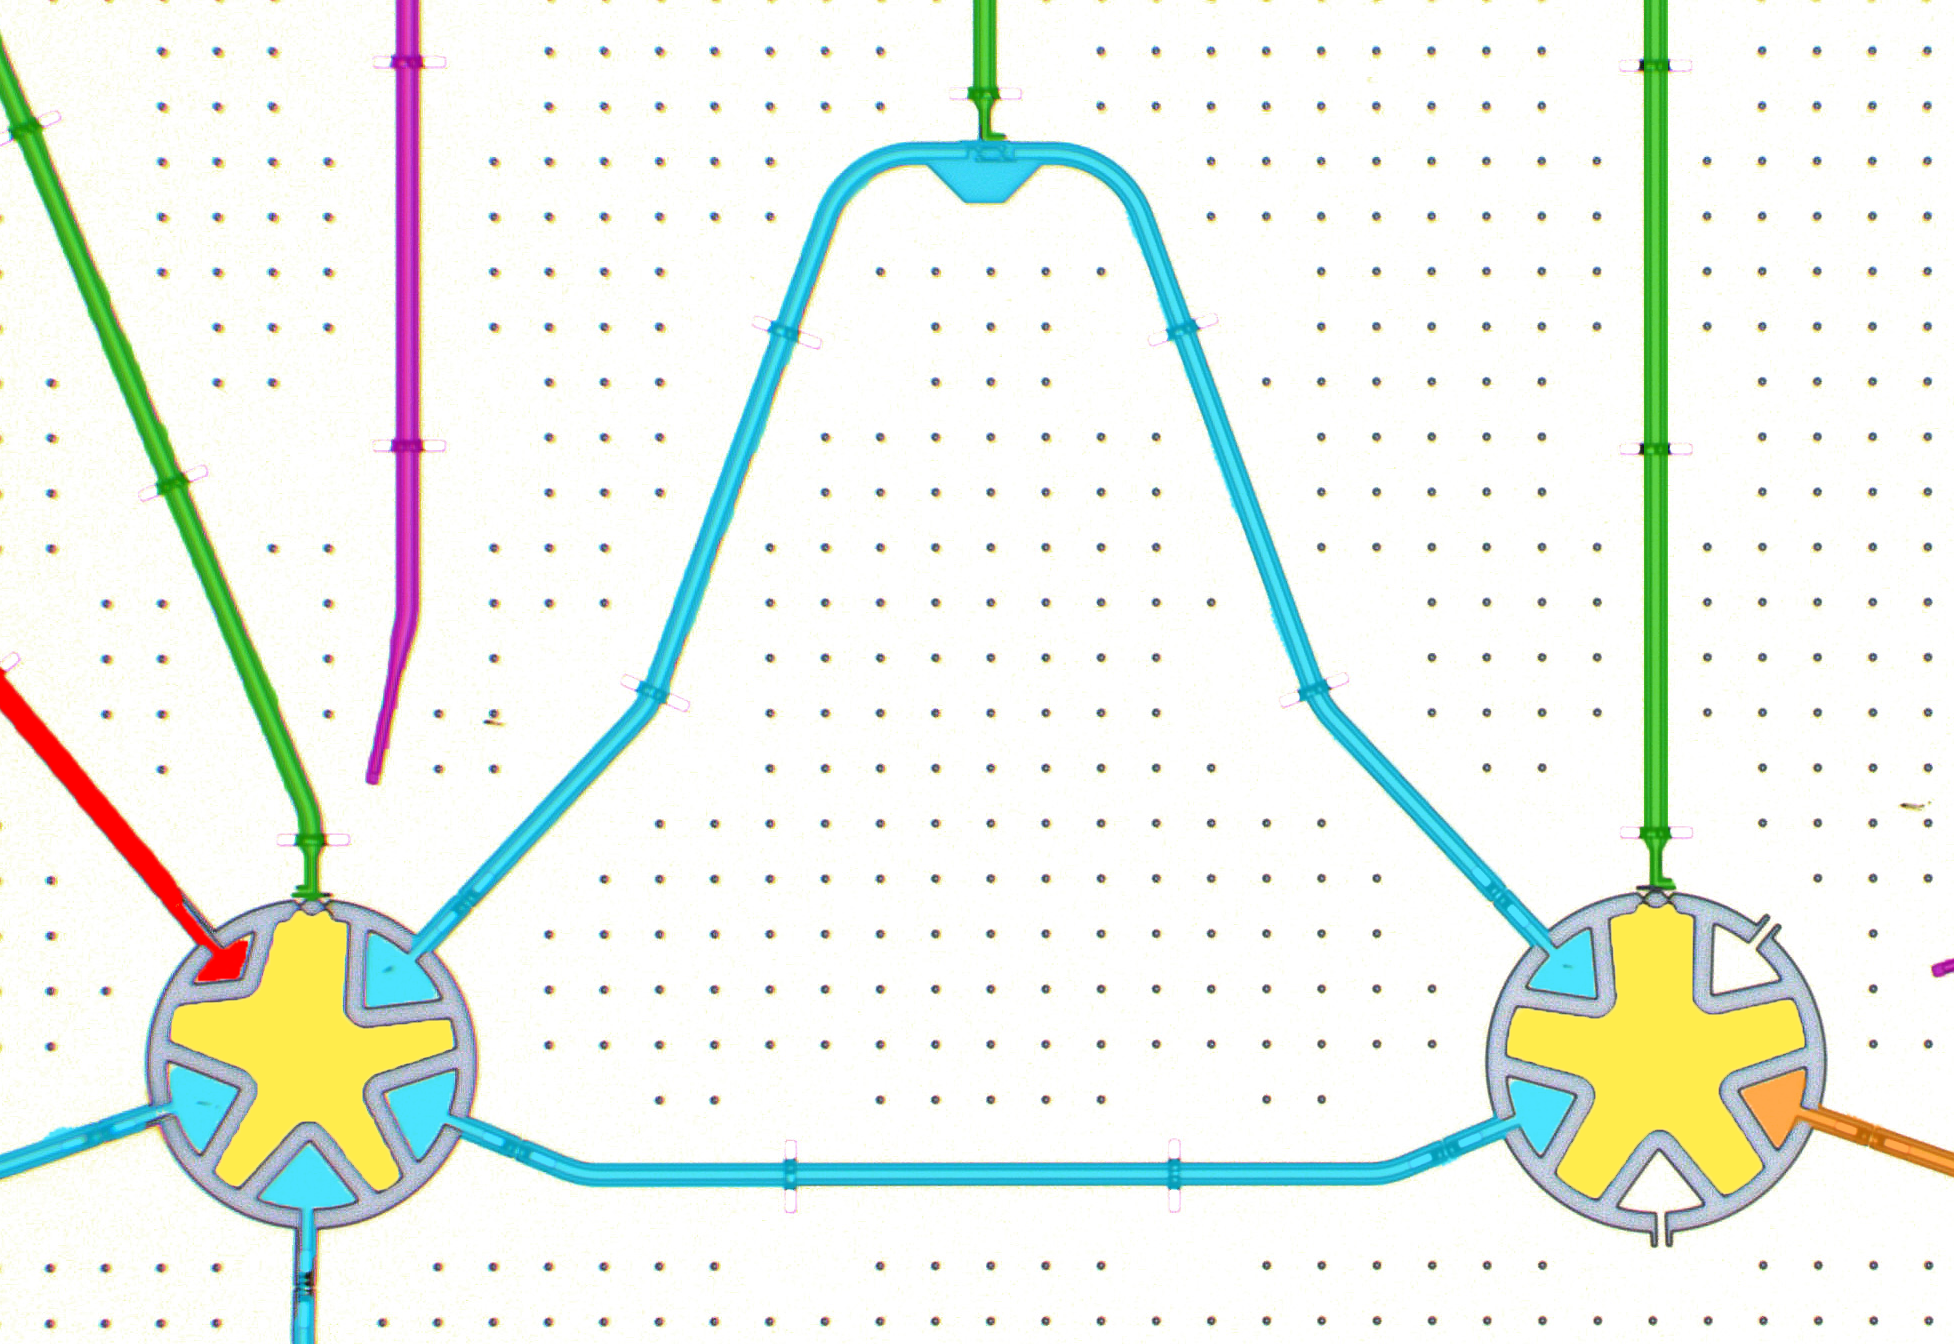
\includegraphics[width=\textwidth]{Images/Chap1/tun_couplers.png} 
        \caption{Micrograph}
        \label{fig:tun_coupl_real}
    \end{subfigure}
    \caption{Two qubits connected by tunable couplers}
    \label{fig:tun_coupl_tot}
\end{figure}

We employ \emph{tunable couplers} \cite{tun_coupler} to control interactions between pairs of qubits.
They allow us to mediate interaction between the qubits and perform two-qubits gates.
They are composed of two coplanar waveguides (see \cref{fig:tun_coupl}).
One of them is a normal waveguide, and thus has a fixed coupling term $J_\text{fixed}$.
The other has a SQUID loop and is flux tunable.
Its coupling term $J_\text{tunable}(\phi)$ can be tuned with the magnetic flux generated by a flux line and going into a SQUID loop placed on the waveguide.

The SQUID loop connected to the coupler allows us to control the interaction between the two qubits. 
To minimise the interaction between the two qubits and the ZZ crosstalk, the DC flux driving the SQUID loop has to be calibrated to the operation point.

To implement a two-qubit gate, a sinusoidal pulse is sent on top of the DC flux to the SQUID loop. If the modulation frequency of this pulse matches a transition of the two-qubit system, it will perform a two-qubit gate.
In this way we are able to turn on interactions between specific levels of the qubits (see \cref{chap:2_qubit_gates}).

\subsection{Emitter Qubits}
Each storage qubit is connected to an emitter qubit, denoted by an ‘E' in the diagram, through tunable couplers ($\text{C}_1$ and $\text{C}_2$).
They have a very strong coupling to a waveguide referred to as \emph{emission line}.
This leads to a rapid decay of any excitation induced in them via the emission line, manifesting as photons travelling through the waveguide.
This prevents us from conducting multiple operations on these qubits, since any excitation would be promptly released into the emission line.
Finding a good DC flux for the tunable couplers linking storage and emitter qubits is crucial to avoid the decay of the former into the latter and subsequently into the emission line, causing the irreversible loss of the quantum state.
